\documentclass[11pt,a4paper]{article}
\usepackage{hyperref}
\usepackage{graphicx}
\usepackage{epsfig}
\begin{document}
\begin{titlepage}
\title{\textbf{Software Requirements Specification}\\Computer Science Marks System\\ \small Version: 0.1\\ }

\author{\\Moeletji Semenya 12349136\\
\textit{For:} \\Mr. Jan Kroeze (University of Pretoria)}



\maketitle
\end{titlepage}
\pagebreak
\tableofcontents
\pagebreak
\section{UI Screen Designs and User Work-Flow Specification}
This section will look at how the system will be used by the different users. Each functional requirement will be accompanied by the appropriate screen designs(The web and mobile user interfaces). 
\subsection{Log In}
		\begin{figure}[h]
		\centering
		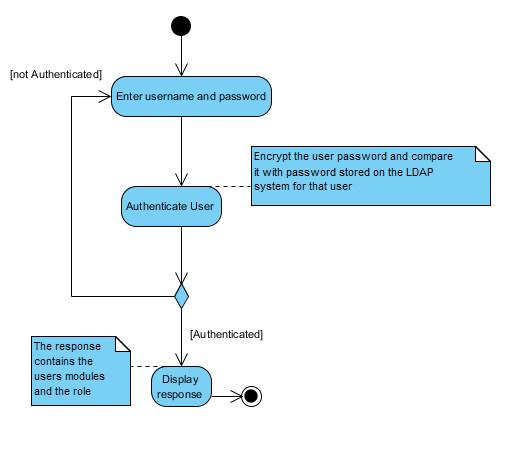
\includegraphics[width=0.7\linewidth]{./uml_login}
		\caption{User log in activity diagram.}
		\label{fig:uml_login}
		\end{figure}

The activity diagram above is a abstract depiction of what will happen when a user logs into the system. After the user gets authenticated by the system, the authentication response object will contain the users information(the modules and roles) as shown in Figure 3 and 5.

\pagebreak

\subsubsection{Mobile Interface Screen Designs}
		\begin{figure}[h]
		\centering
		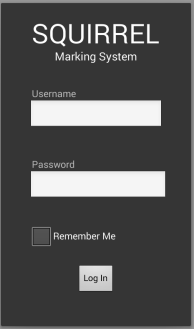
\includegraphics[width=0.7\linewidth,height=15cm]{./mobile_login}
		\caption{The mobile log in screen design.}
		\label{fig:mobile_login}
		\end{figure}

\pagebreak

		\begin{figure}[h]
		\centering
		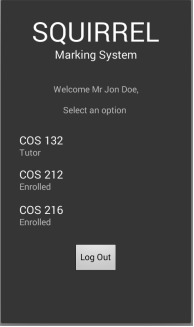
\includegraphics[width=0.7\linewidth, height=15cm]{./mobile_welcomeScreen}
		\caption{Screen design of a successfull log in request.}
		\label{fig:mobile_welcomeScreen}
		\end{figure}
		Figure 3 shows the modules the user is associated with and the roles users have for particular module. 

\pagebreak

\subsubsection{Web Interface Screen Designs}
		\begin{figure}[h]
		\centering
		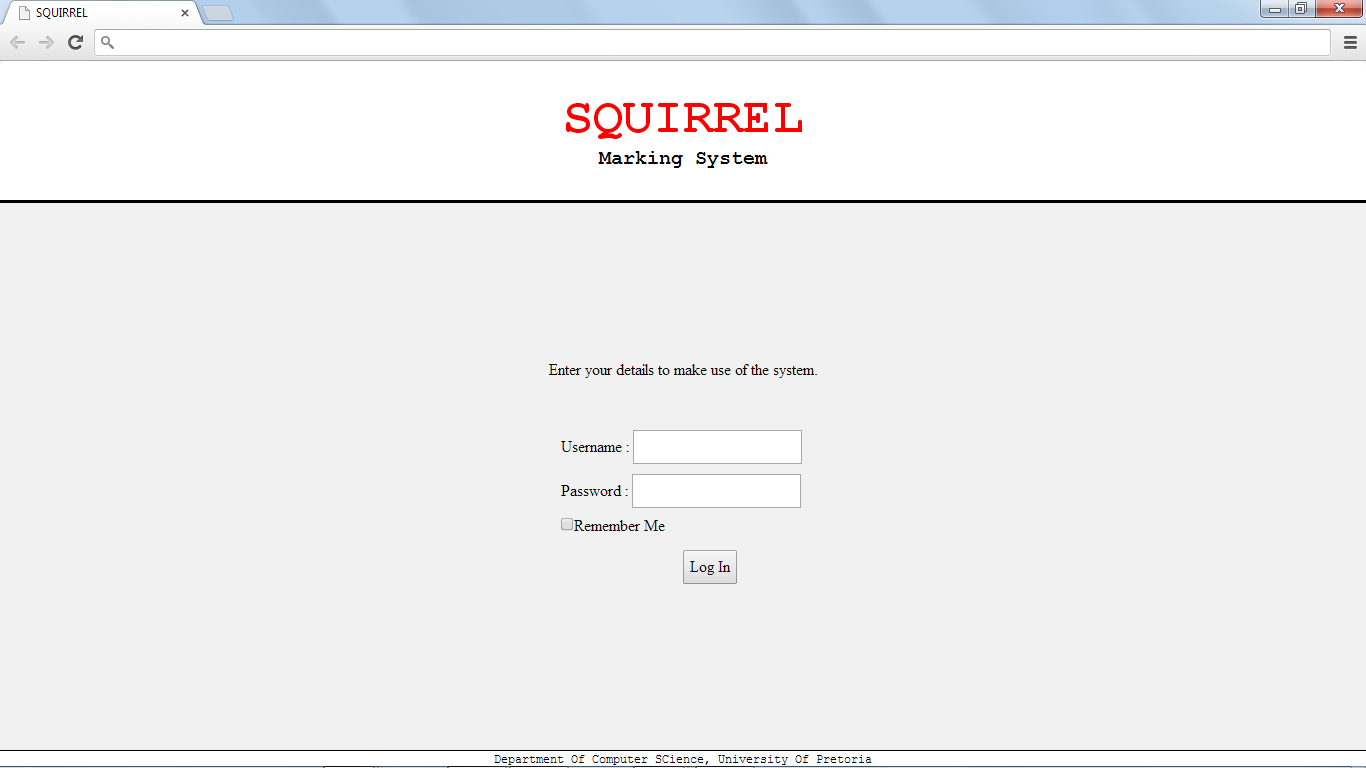
\includegraphics[width=1.0\linewidth]{./web_login}
		\caption{Screen design for web interface}
		\label{fig:web_login}
		\end{figure}
		
\begin{figure*}[h!]
\centering
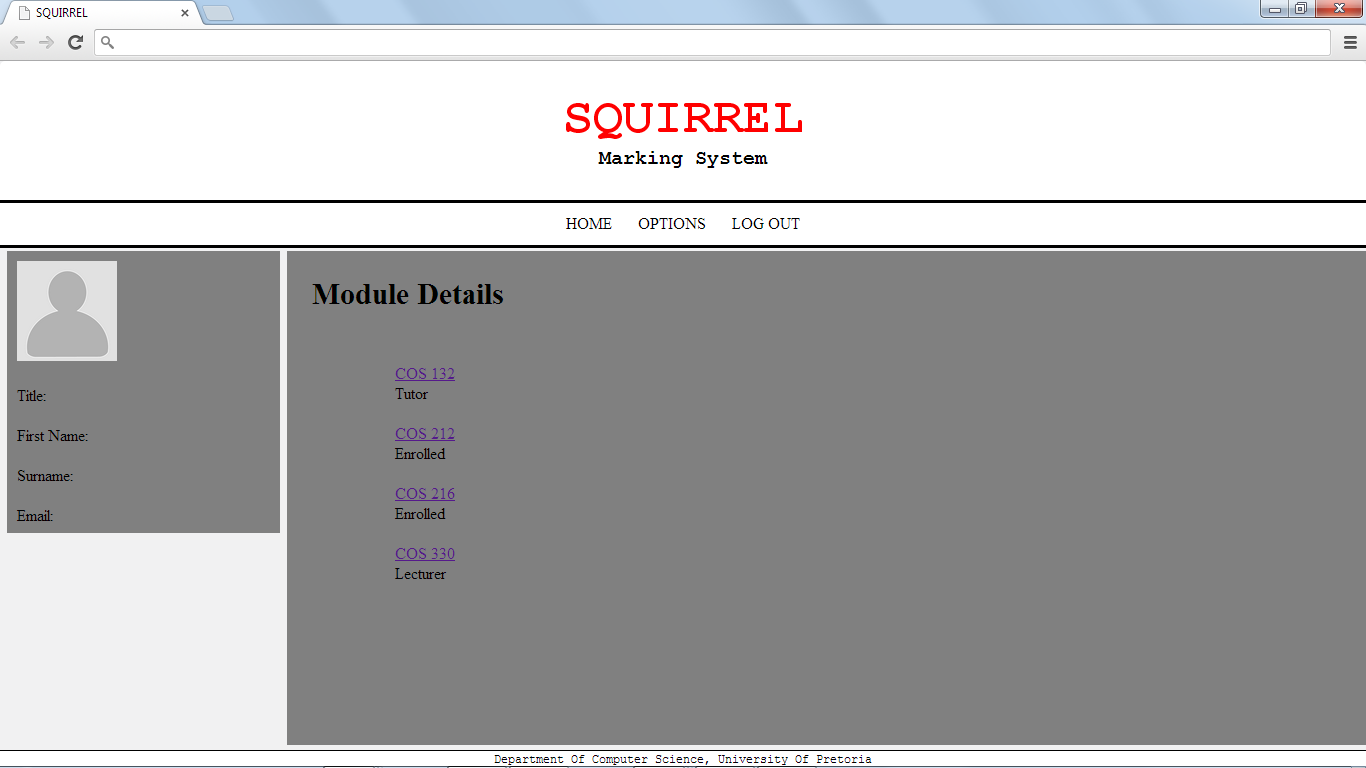
\includegraphics[width=1.0\linewidth]{./web_modules&roles}
\caption{This is the welcome page the user sees after successfully being authenticated.}
\label{fig:web_modules&roles}
\end{figure*}

\pagebreak

\subsection{Assessment Creation}
		\begin{figure}[h]
		\centering
		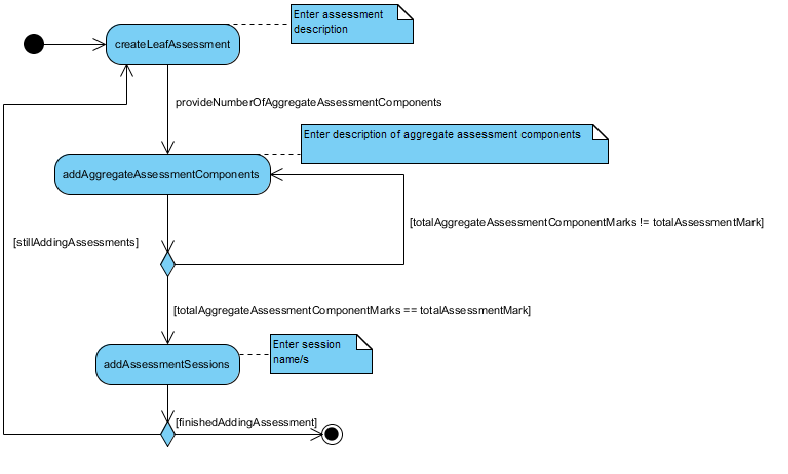
\includegraphics[width=1.0\linewidth]{./uml_assessmentCreation}
		\caption{Activity diagram for creating atomic leaf assessments, aggregate assessments as well as sessions for the atomic assessments.}
		\label{fig:uml_assessmentCreation}
		\end{figure}

	The assessment creation operation is only available to lecturers and only has the web interface as shown below.
	
\pagebreak	
\subsubsection{Web Interface Screen Designs}
\begin{figure*}[h!]
\centering
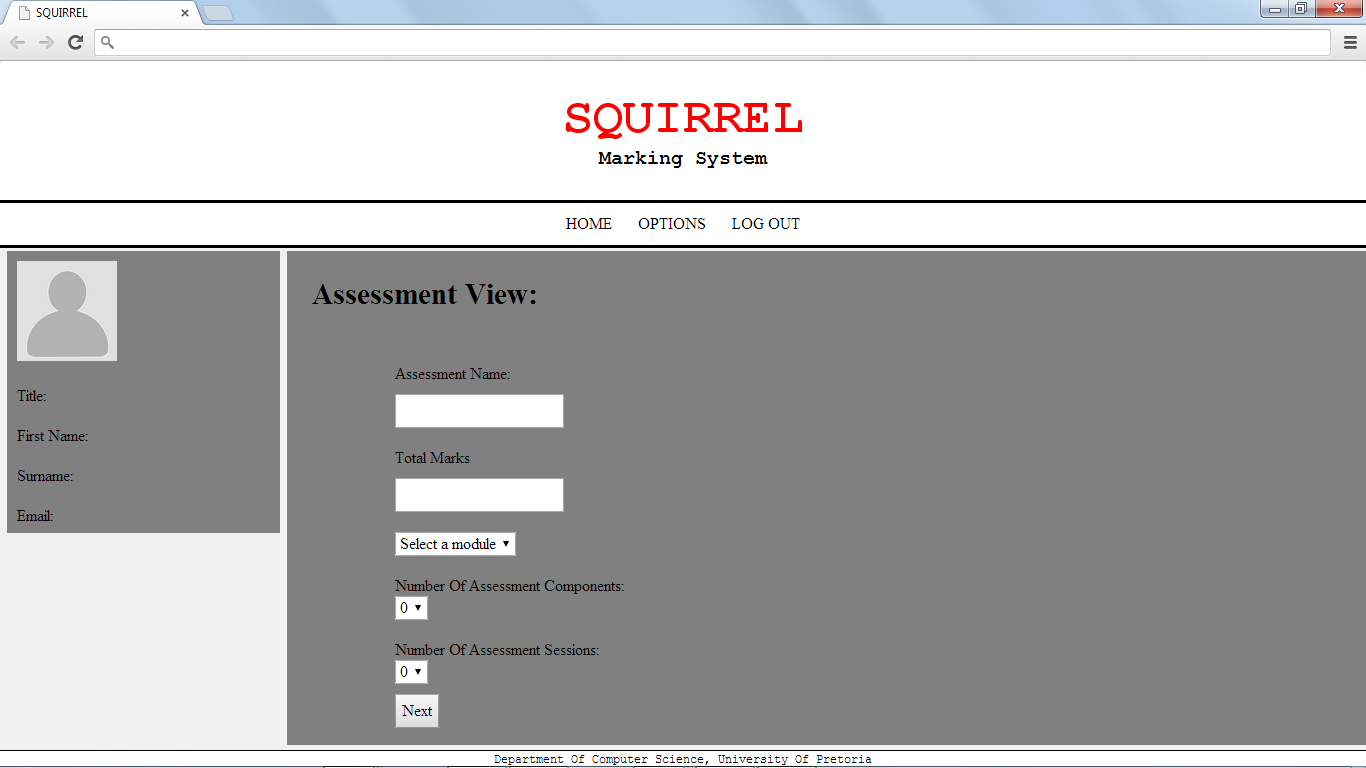
\includegraphics[width=1.0\linewidth]{./web_assessmentView}
\caption{Screen design for creating an atomic assessment.}
\label{fig:web_assessmentView}
\end{figure*}


		\begin{figure*}[h!]
		\centering
		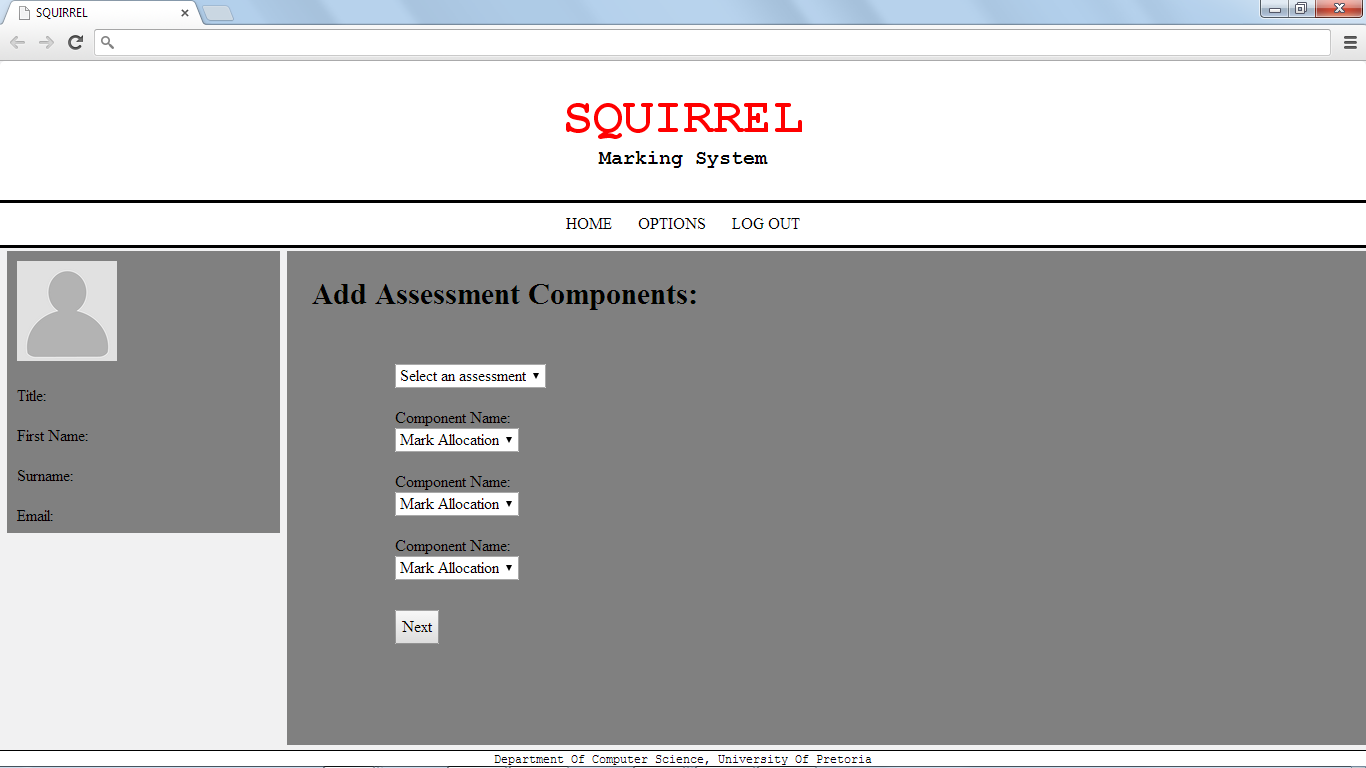
\includegraphics[width=1.0\linewidth]{./web_assessmentComponent}
		\caption{Screen design for adding aggregate assessments.}
		\label{fig:web_assessmentComponent}
		\end{figure*}

\pagebreak
\begin{figure*}[h!]
\centering
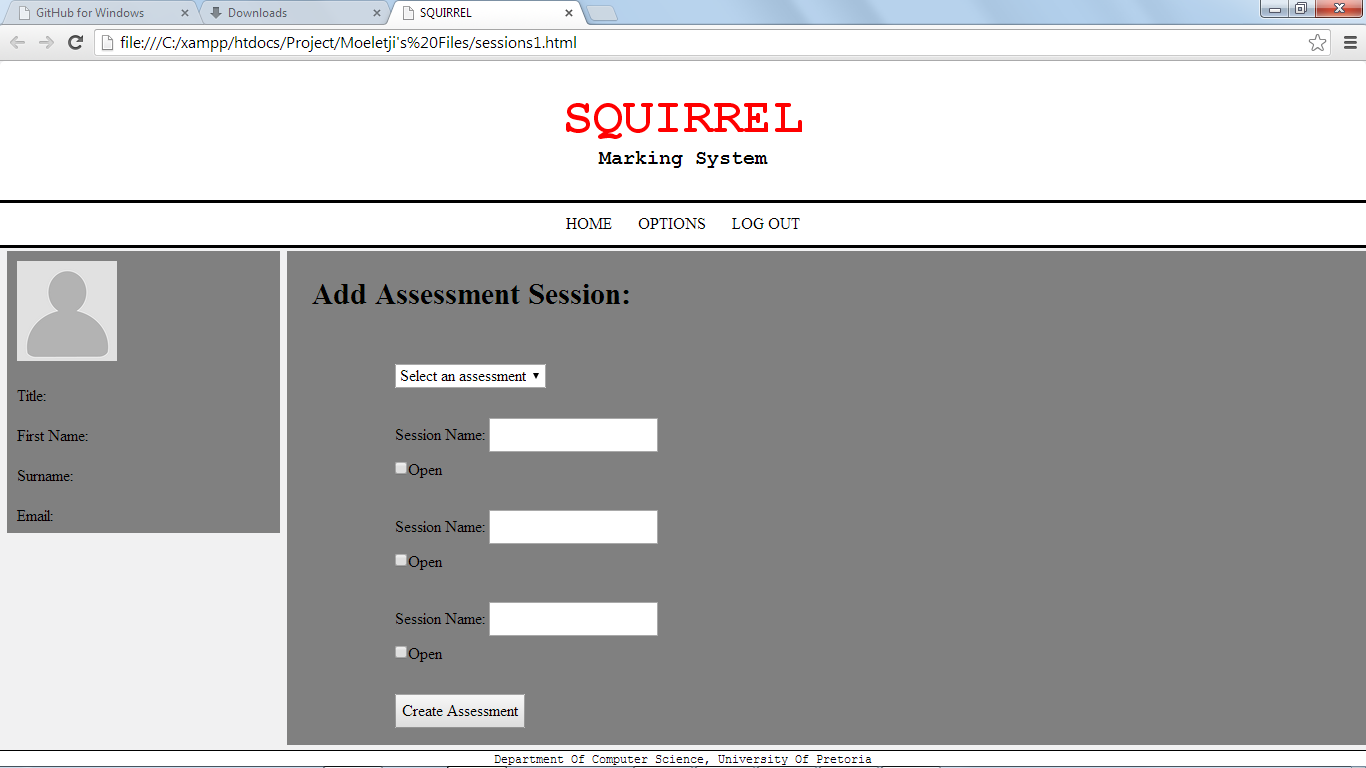
\includegraphics[width=1.0\linewidth]{./web_assessmentSession}
\caption{Screen design for adding sessions for an atomic assessment.}
\label{fig:web_assessmentSession}
\end{figure*}


\subsection{Marks Management}

	\begin{figure*}[h!]
	\centering
	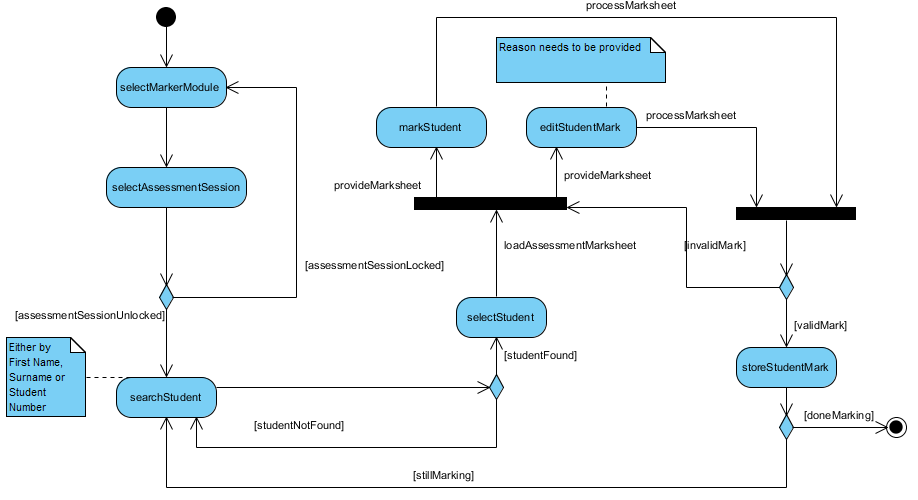
\includegraphics[width=1.0\linewidth]{./uml_markManagement}
	\caption{Activity diagram depiction of how a student would get marked.}
	\label{fig:uml_markManagement}
	\end{figure*}
		
	The activity diagram(Figure 10) depicts how a marker would go about marking a student. The activity diagram is closely linked with the screen designs as it shows how the user would go about marking a student.
\pagebreak
\subsubsection{Mobile Interface Screen Designs}

		\begin{figure*}[h!]
		\centering
		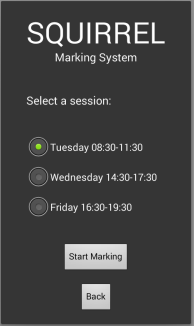
\includegraphics[width=0.7\linewidth]{./mobile_selectSession}
		\caption{Screen design of assessment sessions.}
		\label{fig:mobile_selectSession}
		\end{figure*}
\pagebreak			
		\begin{figure*}[h!]
		\centering
		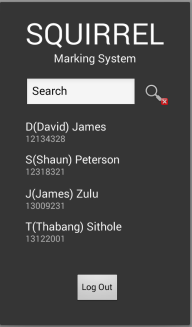
\includegraphics[width=0.7\linewidth]{./mobile_searchForStudent}
		\caption{Screen design of how the students would be displayed and search for on the system.}
		\label{fig:mobile_searchForStudent}
		\end{figure*}
\pagebreak	
		\begin{figure*}[h!]
		\centering
		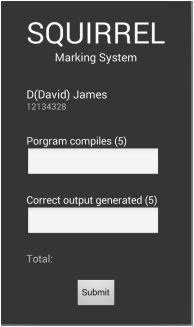
\includegraphics[width=0.7\linewidth]{./mobile_markStudent}
		\caption{Screen design of the interface used to enter student marks.}
		\label{fig:mobile_markStudent}
		\end{figure*}
\pagebreak	

\subsubsection{Web Interface Screen Designs}
\begin{figure*}[h!]
\centering
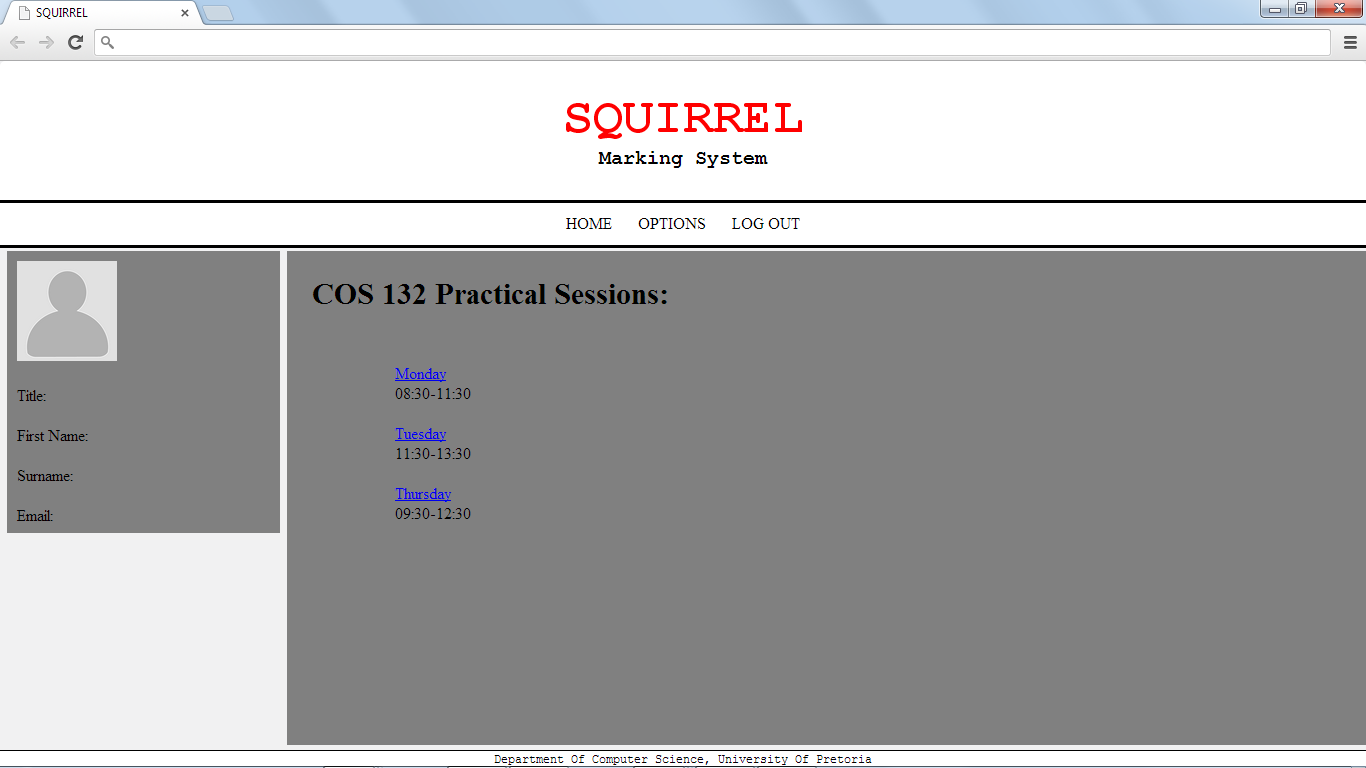
\includegraphics[width=1.0\linewidth]{./web_markerSessions}
\caption{List of available marking sessions.}
\label{fig:web_markerSessions}
\end{figure*}
		
		\begin{figure*}[h!]
		\centering
		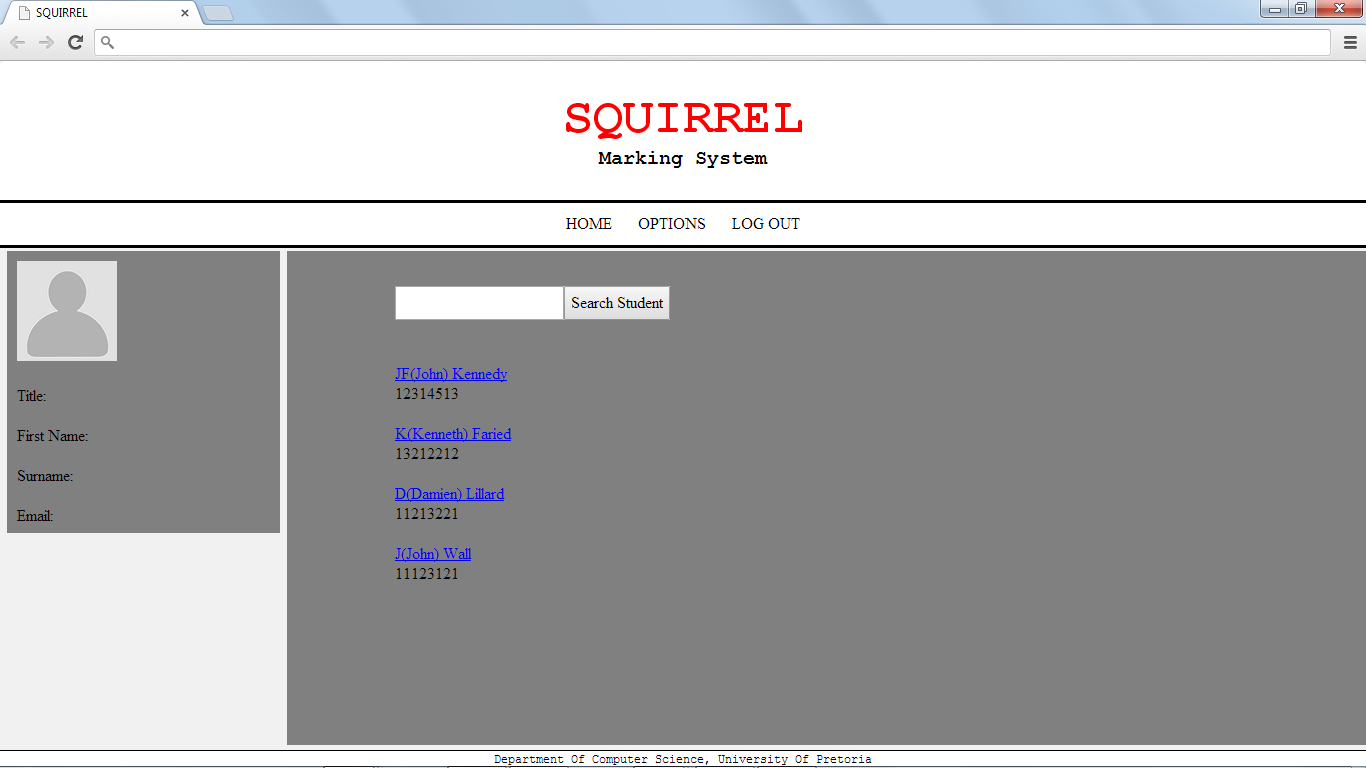
\includegraphics[width=1.0\linewidth]{./web_searchStudent}
		\caption{List of students in the sessions who need to be marked.}
		\label{fig:web_searchStudent}
		\end{figure*}
		
\pagebreak
				\begin{figure*}[h!]
				\centering
				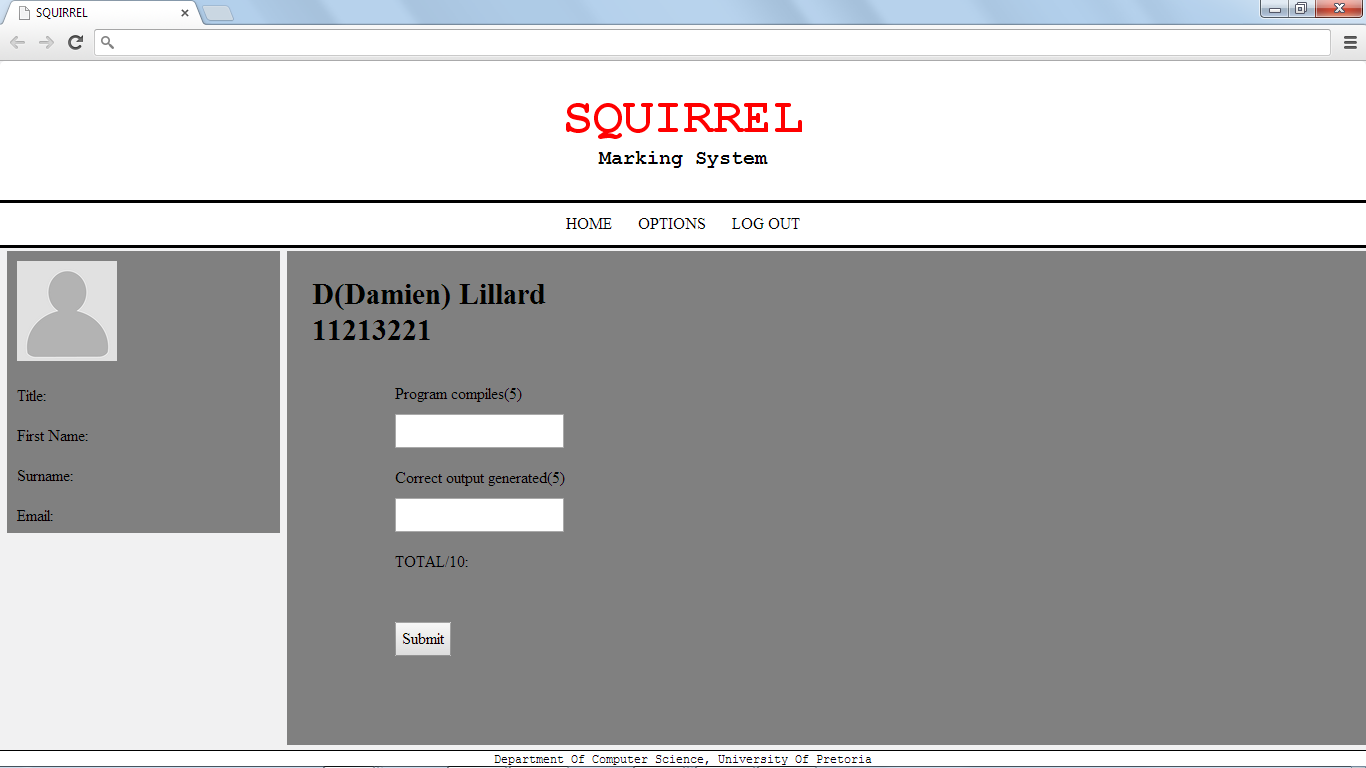
\includegraphics[width=1.0\linewidth]{./web_markStudent}
				\caption{A student being marked.}
				\label{fig:web_markStudent}
				\end{figure*}

\subsection{Reporting}
	\begin{figure}[h]
	\centering
	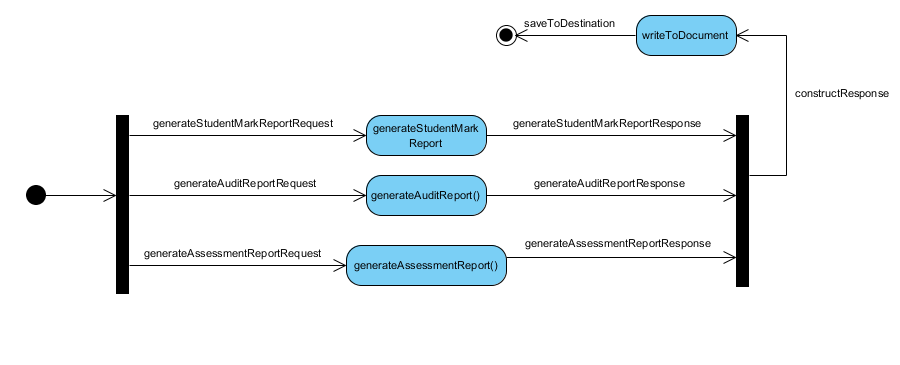
\includegraphics[width=1.0\linewidth]{./uml_reportGenerating}
	\caption{Activity diagram of how reports would be generated by users.}
	\label{fig:uml_reportGenerating}
	\end{figure}
Students wll be able to generate their mark reports on either platform(mobile or web interface), while lecturers will only be able to generate assessment and audit reports via the web interface.
\pagebreak
\subsubsection{Mobile Interface Screen Designs}

	\begin{figure}[h]
	\centering
	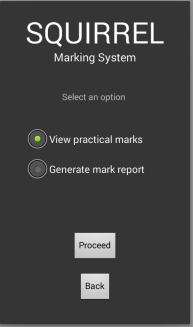
\includegraphics[width=0.7\linewidth]{./mobile_studentViewOption}
	\caption{Options of reports a student can generate.}
	\label{fig:mobile_studentViewOption}
	\end{figure}
\pagebreak
		\begin{figure}[h]
		\centering
		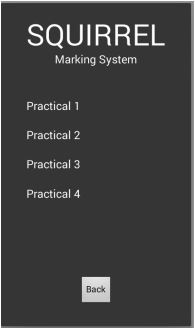
\includegraphics[width=0.7\linewidth]{./mobile_practicalsView}
		\caption{List of practicals.}
		\label{fig:mobile_practicalsView}
		\end{figure}

\pagebreak
	\begin{figure}[h]
	\centering
	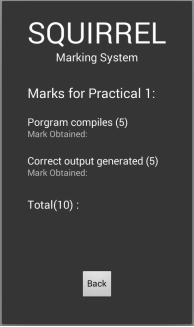
\includegraphics[width=0.7\linewidth]{./mobile_pracMarksheet}
	\caption{Screen design of a report for a students practical 1.}
	\label{fig:mobile_pracMarksheet}
	\end{figure}
\pagebreak		
	\begin{figure}[h]
	\centering
	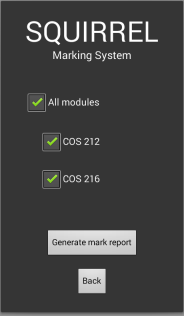
\includegraphics[width=0.7\linewidth]{./mobile_studentReport}
	\caption{Screen design for generating a students' mark report. }
	\label{fig:mobile_studentReport}
	\end{figure}	
\pagebreak	
\subsubsection{Web Interface Screen Designs}
\begin{figure*}[h!]
\centering
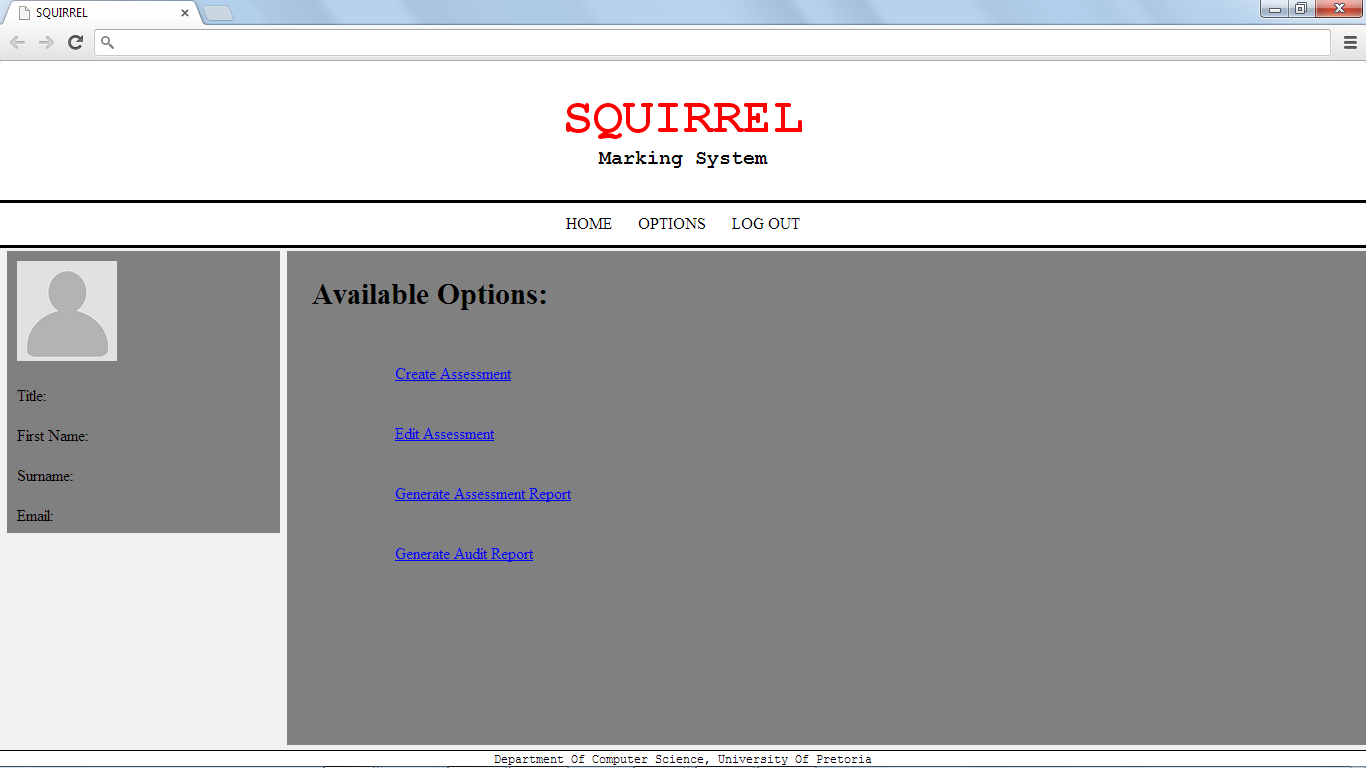
\includegraphics[width=1.0\linewidth]{./web_lecturerOptions}
\caption{Report options lecturers have.}
\label{fig:web_lecturerOptions}
\end{figure*}

		\begin{figure*}[h!]
		\centering
		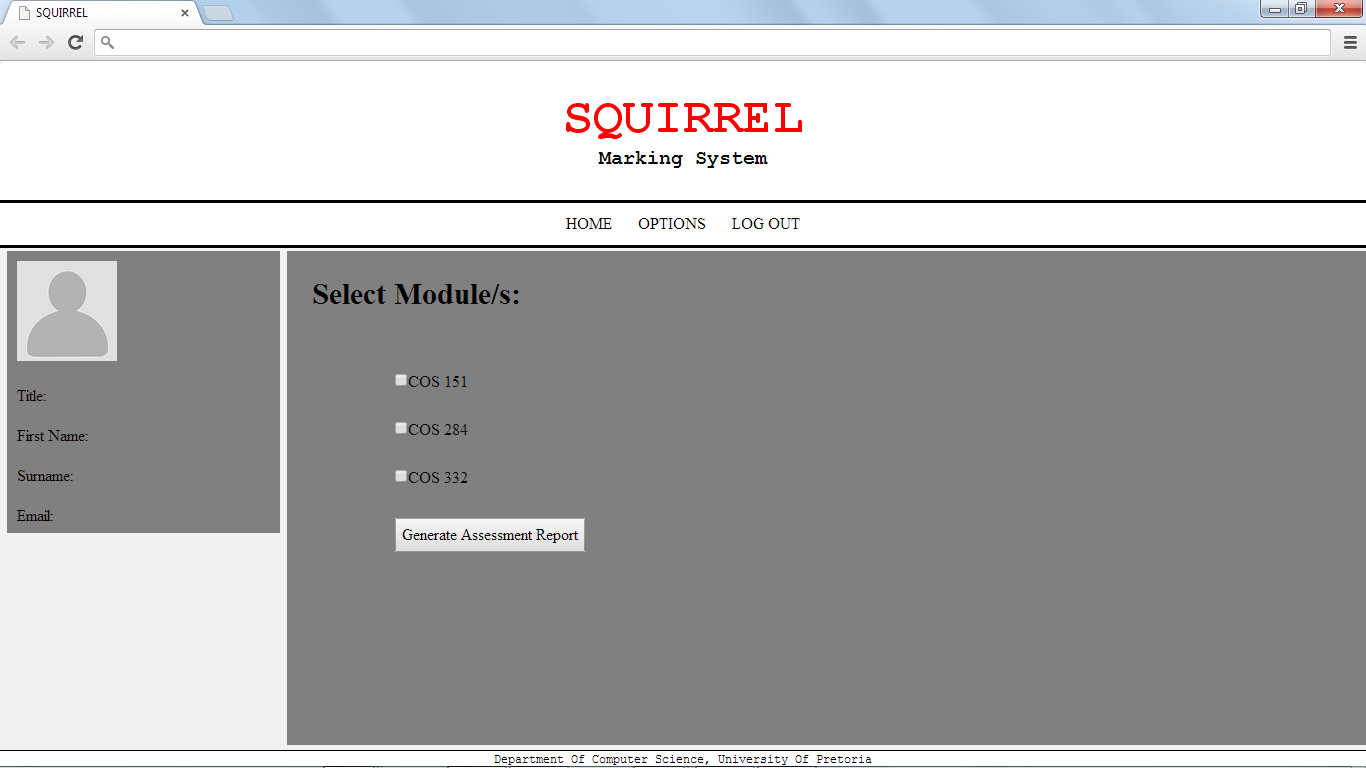
\includegraphics[width=1.0\linewidth]{./web_assessmentReport}
		\caption{Screen design for generating assessment reports.}
		\label{fig:web_assessmentReport}
		\end{figure*}

					\begin{figure}[h]
					\centering
					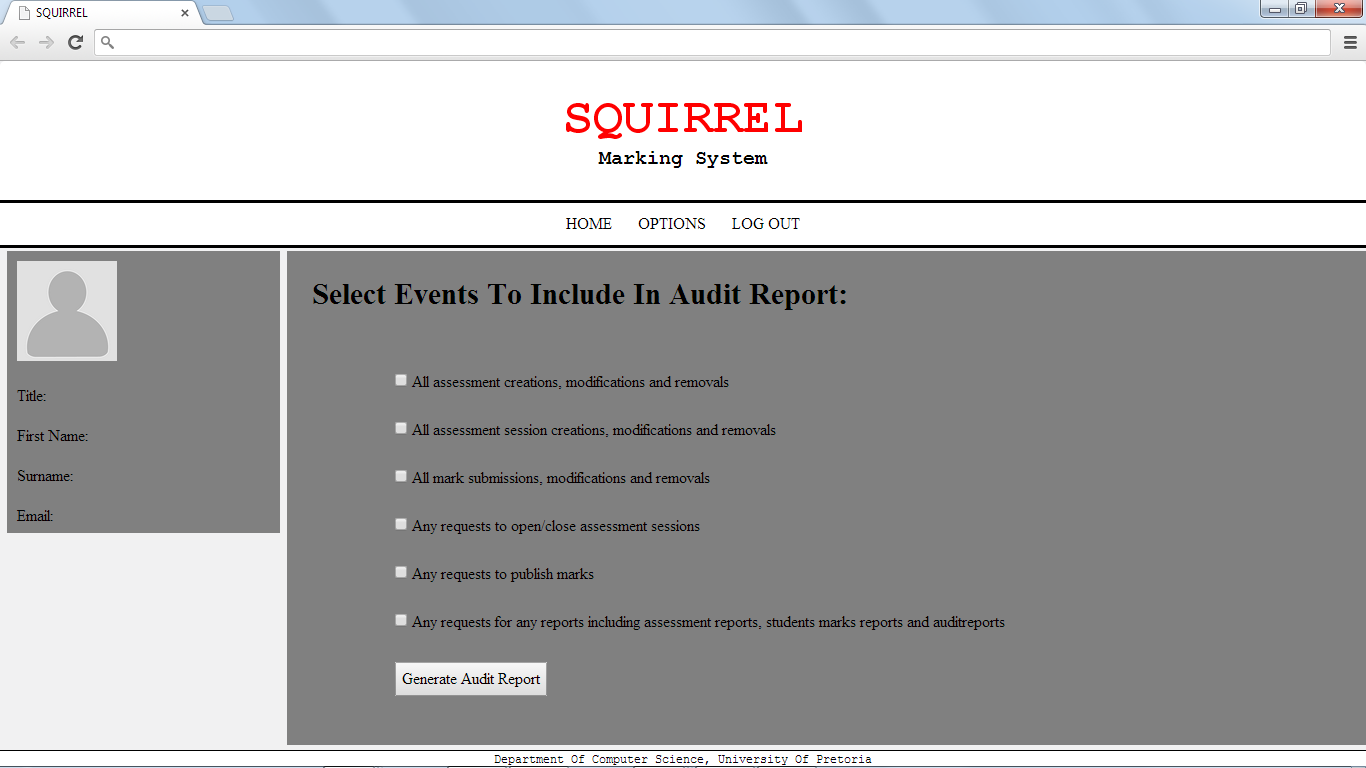
\includegraphics[width=1.0\linewidth]{./web_auditReport}
					\caption{Screen design for generating audit reports.}
					\label{fig:web_auditReport}
					\end{figure}
			
\end{document}
